\chapter{El llenguatge Quadriga}
\label{chap:llenguatgeQ}

\section{Estructura dels programes}

Un programa fet amb Quadriga consta de diferents elements (Component, Sistema, Event, Thread, Prototip, Main) distribuïts en diferents fitxers o paquets. El concepte de paquets està directament agafat de {\em Java} i serveix per a crear espais de noms, tal que un programador sigui lliure de crear elements amb el nom que vulgui, que sempre seran compatibles amb altres amb el mateix nom, però diferent paquet.

Cada paquet de Quadriga està representat per un fitxer. Els fitxers de quadriga acaben en {\em \"{}.qdg\"{}}. Si un paquet es diu {\em \"{}tetris.input\"{}} aleshores el fitxer serà anomenat {\em \"{}tetris/input.qdg\"{}}. Aquesta metodologia permet al compilador trobar fàcilment els arxius que necessita. En quadriga no existeix cap ordre per incloure fitxers externs. En comptes d'això, cal declarar els elements que es necessiten, i el compilador els buscarà als directoris d'inclusió. Si per exemple volem fer servir el {\em Component Transform} del paquet {\em cat.quadriga.base} aleshores hem de declarar {\em @component cat.quadriga.base.Transform} abans de fer-lo servir, i el compilador ja s'encarregarà de trobar-lo. Aquesta sentència es pot usar per predeclarar un element del mateix fitxer abans d'on està pròpiament escrit per tal d'utilitzar-lo, de forma similar a com ho fa {\bf C}. Per tal d'importar una classe de {\em Java} cal usar la paraula clau {\bf @java} tal com s'importen la resta d'elements. Com a java, es considera que les classes del paquet {\em java.lang} estan automàticament importades.

El llenguatge utilitza essencialment la mateixa estructura que Java, amb la diferència que a Quadriga no es creen classes, sinó els elements propis: {\em Components, Sistemes, Events, Threads, Prototips i Mains}. També s'han afegit algunes instruccions extres. Totes les paraules clau pròpies de {\em Quadriga} comencen amb el símbol {\bf @}.

\subsection{Entitat}

\begin{verbatim}
Entity<Component1, Component2, ...>
\end{verbatim}

Una entitat, en Quadriga, és simplement un tipus de variable o paràmetre. Com que cada entitat està identificada pels seus components, es permet de nombrar quins components se suposa que té associats de forma similar a com es fan els {\em Generics} en Java.

\section{Declaració de tipus de dades}

\subsection{Components}

%\begin{verbatim}
%@component Puntuació {
%  *CTaulell;
%  int punts  = 0;
%  int línies = 0;
%  int nivell = 0;
%}
%\end{verbatim}

\begin{figure}[h!]
  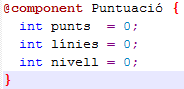
\includegraphics{./img/ExempleComponent.png}
  \caption{Component}
\end{figure}

La declaració d'un Component comença amb la paraula clau {\em \"{}@component\"{}} seguida de l'identificador desitjat del component. Seguidament, dintre de claus (\{ \}), es declaren les variables d'estat de forma similar a Java, amb la possibilitat d'establir un valor inicial si es desitja, tal com es mostra en l'exemple.

També dintre de les claus, i a l'inici es pot especificar quins Components necessita aquest Component (requisits previs), afegint un asterisc {\bf *} i el nom d'aquests components.

Els tipus permesos són els tipus primitius de Java (byte, short, int, long, float, double, boolean, char) i classes que siguin {\em Serialitzables}.

\subsection{Events}

%\begin{verbatim}
%@event NovaPeça {
%  int tipus;
%}
%\end{verbatim}

\begin{figure}[h!]
  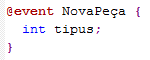
\includegraphics{./img/ExempleEvent.png}
  \caption{Event}
\end{figure}

Un event es declara de forma idèntica a un component, a excepció de la paraula clau inicial {\em \"{}@component\"{}} que és substituïda per {\em \"{}@event\"{}}; i no hi ha \"{}requisits\"{}.

\subsection{Sistemes}

%\begin{verbatim}
%@system LògicaPeça {
%  @components {
%    CPeça
%  }
%  
%  @init {...}
%  
%  @cleanUp {...}
%  
%  @update(Entity<CPeça> entitat: ENTITY, float dt : DELTA_TIME) {...}
%  
%  @newEntity(Entity<CPeça> entitat: ENTITY) {...}
%  
%  @eraseEntity(Entity<CPeça> entitat: ENTITY) {...}
%  
%  @event NovaPeça(
%                  NovaPeça event: EVENT, 
%                  Entity<CPeça> entitat: ENTITY
%                  )
%  {...}
%  
%  @event ELeft(Entity<CPeça> entitat: ENTITY) {...}
%  
%  @event ERight(Entity<CPeça> entitat: ENTITY) {...}
%  
%  @event EDown(Entity<CPeça> entitat: ENTITY) {...}
%  
%  @event ETurnL(Entity<CPeça> entitat: ENTITY) {...}
%  
%  @event ETurnR(Entity<CPeça> entitat: ENTITY) {...}
%}
%\end{verbatim}

\begin{figure}[h!]
  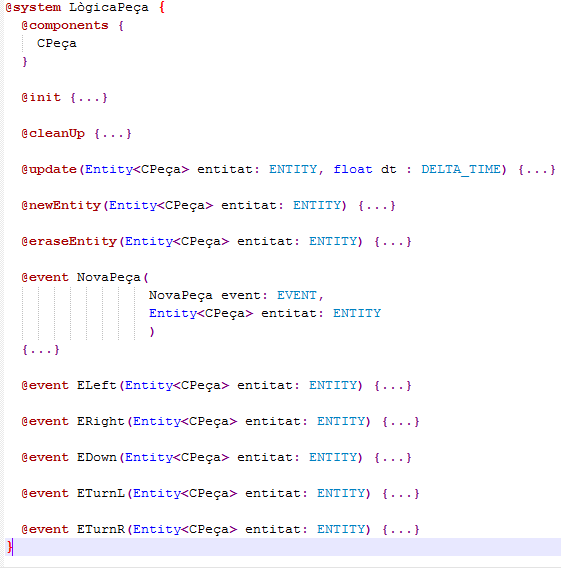
\includegraphics{./img/ExempleSystem.png}
  \caption{Sistema}
\end{figure}

La declaració d'un Sistema comença de forma similar a la d'un component, amb la paraula clau {\em \"{}@system\"{}}, el nom del sistema, i els diferents elements d'aquest. El primer element que cal introduir sempre, i l'únic obligatori, és la llista de components que una Entitat necessita tenir per que aquest sistema l'afecti. Aquesta llista se situa entre claus, tal com es mostra a la figura \ref{fig:ExempleSystem2}

%\begin{verbatim}
%  @components { }
%\end{verbatim}

\begin{figure}[h!]
  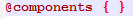
\includegraphics{./img/ExempleSystem2.png}
  \caption{Declaració dels components necessaris \label{fig:ExempleSystem2}}
\end{figure}

Els elements de la llista poden anar separats de punts i coma ({\bf ;}), però poden estar separats únicament per espais.

A continuació vindran les funcions del sistema. Les dues primeres a destacar són {\bf @init} i {\bf @cleanUp}. Aquestes s'executen a l'inici i a la fi de l'execució, una única vegada. Entre 2 sistemes, l'ordre de en que s'executin aquestes funcions depèn únicament de l'ordre en el qual s'han declarat en un Thread. Si 2 Threads declaren el mateix sistema, aquest s'executarà dues vegades.

La funció més important d'un sistema és normalment la funció {\bf @update}. Aquesta funció s'executa un cop per {\em tick} del joc. En el pas de paràmetres cal comentar la introducció del concepte de {\bf semàntiques}. Aquestes semàntiques s'indiquen després de cada paràmetre usant el símbol dos punts {\bf :}. El tipus de paràmetre cal que sigui compatible amb la semàntica. En el cas de la funció {\bf @update} se'n proporcionen 2:

\begin{itemize}
  \item {\bf ENTITY}: Correspon a la entitat actualitzada.
  \item {\bf DELTA\_TIME}: És el temps, en segons, des de la última vegada que es va cridar la funció per la mateixa entitat.
\end{itemize}

Les següents funcions són {\bf @newEntity} i {\bf @eraseEntity}, que es criden quan una entitat té per primera vegada els components necessaris o deixa de tenir-los, respectivament. Aquestes funcions només proporcionen la semàntica {\bf ENTITY}.

Finalment hi ha les funcions que tracten events. Aquestes funcions comencen amb la paraula clau {\bf @event}, seguida de l'identificador de l'event que es vol tractar. Quan una entitat que pertany al sistema rebi l'event, automàticament es cridarà aquesta funció. A part de la semàntica {\bf ENTITY}, es proporciona la semàntica {\bf EVENT}, que ha de tenir el mateix tipus que l'event tractat i proporcionarà totes les dades que vinguin amb aquest event.

\subsection{Prototips}

%\begin{verbatim}
%@prototype PPeça(Entity<Puntuació> taulell)
%{
%  Transform()
%  CPeça(taulell: taulell)
%  @child {
%    "cub1" : CubDeTaulell(posX:0, posY:0, color: 1)
%    "cub2" : CubDeTaulell(posX:0, posY:0, color: 1)
%    "cub3" : CubDeTaulell(posX:0, posY:0, color: 1)
%    "cub4" : CubDeTaulell(posX:0, posY:0, color: 1)
%  }
%}
%\end{verbatim}

\begin{figure}[h!]
  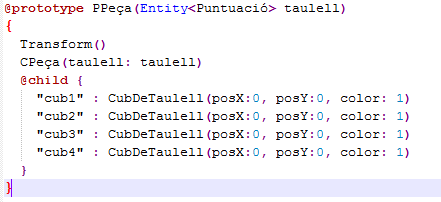
\includegraphics{./img/ExemplePrototype.png}
  \caption{Prototip}
\end{figure}

L'estructura d'un prototip és una mica més complexa. Primer cal especificar-ne el nom, seguit dels paràmetres que té el prototip. Després se li afegeixen un seguit de plantilles per a dues coses: Components que tindrà l'entitat, i altres entitats filles que crearà. Els elements sempre es creen i afegeixen en l'ordre establert.

Per a afegir un component, simplement cal escriure el nom i, entre parèntesi, donar valor als camps. Per fer-ho, només cal escriure el nom del camp, dos punts {\bf :} i el valor a assignar-hi. Aquells camps que tinguin valor per defecte no cal que siguin assignats.

Per a especificar Entitats filles, cal especificar-les dintre d'una estructura {\em\"{}@child\{ \}\"{}}. Aquí la fórmula a utilitzar és indicar primer el nom (de forma opcional), a continuació el prototip utilitzat i finalment els paràmetres, de forma similar als Components. Si es vol sobreescriure un valor d'un Component d'algun d'aquests fills, s'haurà d'especificar el nom del component, punt {\bf .} i finalment el camp del component.

Finalment també es pot executar codi si aquest va dintre d'una estructura {\em\"{}@init\{ \}\"{}}, que pot ser repetida diverses vegades al prototip.

\subsection{Threads}

%\begin{verbatim}
%@thread LlogicaTetris {
%  @system SGameOverScreen;
%  @system InputManager;
%  @system LlògicaTaulell;
%  @system LlògicaPeça;
%  
%  @init {...}
%  
%  @cleanUp {...}
%}
%\end{verbatim}

\begin{figure}[h!]
  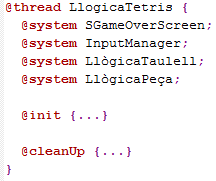
\includegraphics{./img/ExempleThread.png}
  \caption{Thread}
\end{figure}

Un Thread indica quins Sistemes s'executaran, i en quin ordre, i una funció d'Init i CleanUp (opcionals) que s'executaran a l'inici i final de l'execució del programa.

\subsection{Main}

%\begin{verbatim}
%@main Main {
%  @thread SimpleRenderThread
%  @thread LlogicaTetris
%  
%  @init {...}
%  
%  @cleanUp {...}
%}
%\end{verbatim}

\begin{figure}[h!]
  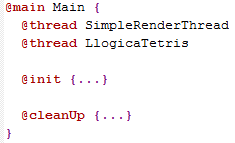
\includegraphics{./img/ExempleMain.png}
  \caption{Main}
\end{figure}

L'objecte Main indica quins Threads s'executen i l'ordre d'aquests (si l'execució no és paral·lela), a més d'un Init i un CleanUp.

\section{Instruccions pròpies}

Aquí es mostraran les instruccions pròpies de Quadriga. Per veure-les degudament remarcades, consultar la figura \ref{fig:ExempleSentencia}.

\subsection{Nova Entitat}

\begin{verbatim}
@newEntity(nom, pare)
\end{verbatim}

Aquesta instrucció retorna una Entitat nova. Se li pot especificar un nom i una Entitat pare, o deixar els paràmetres a null.

\subsection{Eliminar Entitat}

\begin{verbatim}
@eraseEntity entitat;
\end{verbatim}

Elimina una Entitat.

\subsection{Cercar Entitat}

\begin{verbatim}
@find[nom]
\end{verbatim}

Cerca una Entitat amb el nom especificat i sense pare.

\subsection{Aplicar prototip}

\begin{verbatim}
@prototype entitat : nomPrototip( param1: valor1, param2: valor2, 
                                  Component1.camp1: valor3, Component1.camp2: valor4,
                                  ...)
\end{verbatim}

Fa que a una Entitat se li apliqui un Prototip.

\subsection{Agregar Component}

\begin{verbatim}
@add nomComponent(param1: valor1, param2: valor2) : entitat;
\end{verbatim}

Fa que a una Entitat se li agregui un Component.

\subsection{Cridar Event}

\begin{verbatim}
@event[temps] nomEvent(param1: valor1, param2: valor2) : entitat ;
\end{verbatim}

Crida un event. El temps ha de ser positiu, o es pot ometre (per fer una crida instantània), així com la Entitat sobre la que cridar també es pot ometre (fent un Broadcast).

\subsection{Accedir a un Component}

\begin{verbatim}
entitat[Component]
\end{verbatim}

Accedeix a un Component de la Entitat.

\subsection{Accedir a una Entitat filla}

\begin{verbatim}
entitat["nomFilla"]
\end{verbatim}

Accedeix a una Entitat filla amb el nom especificat.

\subsection{Nombre Aleatori}

\begin{verbatim}
@rnd
\end{verbatim}

Retorna un objecte del tipus {\em java.util.Random}.

\begin{figure}[h!]
  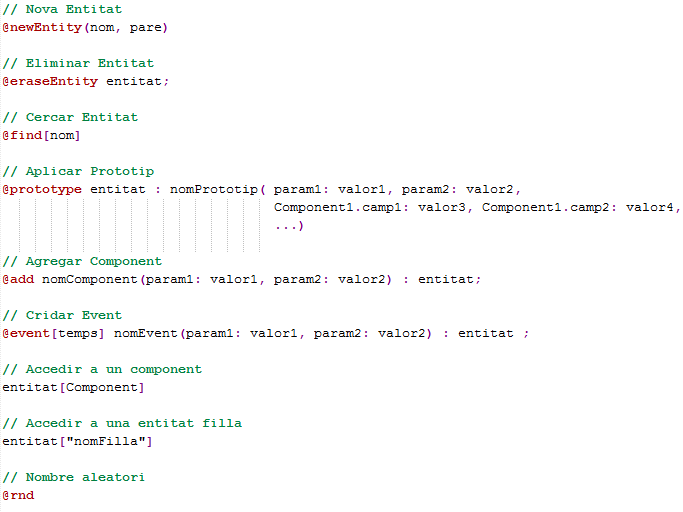
\includegraphics{./img/ExempleSentencies.png}
  \caption{Main \label{fig:ExempleSentencia}}
\end{figure}

\section{Execució}

Per executar un programa de quadriga cal executar la classe {\em cat.quadriga.parsers.Quadriga} amb un únic paràmetre: el nom de l'objecte Main que es vol executar. Cal que Java pugui trobar totes les llibreries Java necessàries (vecmath, hsqldb, lwjgl, slick-util, lwjgl-util) com les llibreries natives de LWJGL.